\documentclass[border=4pt]{standalone}

\usepackage{amsmath}
\usepackage{tikz}
\usepackage{mathdots}
\usepackage{yhmath}
\usepackage{cancel}
\usepackage{color}
\usepackage{siunitx}
\usepackage{array}
\usepackage{multirow}
\usepackage{amssymb}
\usepackage{gensymb}
\usepackage{tabularx}
\usepackage{booktabs}
\usetikzlibrary{fadings}
\usetikzlibrary{patterns}
\usetikzlibrary{shadows.blur}
\usetikzlibrary{shapes}
 

\begin{document}




\tikzset{every picture/.style={line width=0.75pt}} %set default line width to 0.75pt        

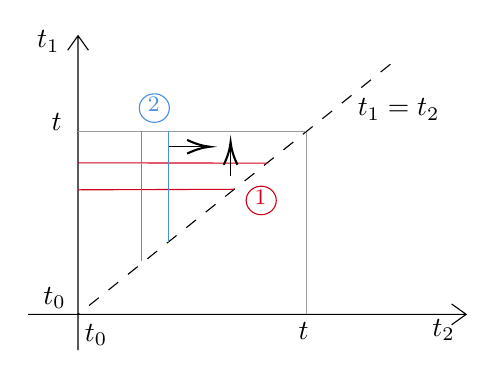
\begin{tikzpicture}[x=0.75pt,y=0.75pt,yscale=-1,xscale=1]
%uncomment if require: \path (0,300); %set diagram left start at 0, and has height of 300

%Shape: Axis 2D [id:dp9797303376366853] 
\draw  (166,200.25) -- (377,200.25)(190,66) -- (190,217.5) (370,195.25) -- (377,200.25) -- (370,205.25) (185,73) -- (190,66) -- (195,73)  ;
%Straight Lines [id:da0694375272829999] 
\draw  [dash pattern={on 4.5pt off 4.5pt}]  (340.5,79.75) -- (190,200.25) ;
%Straight Lines [id:da5775487705604185] 
\draw [color={rgb, 255:red, 155; green, 155; blue, 155 }  ,draw opacity=1 ]   (300,112.25) -- (300,200.25) ;
%Straight Lines [id:da31552104007489645] 
\draw [color={rgb, 255:red, 155; green, 155; blue, 155 }  ,draw opacity=1 ]   (190,112.25) -- (300,112.25) ;
%Shape: Boxed Line [id:dp7433050863727066] 
\draw [color={rgb, 255:red, 208; green, 2; blue, 27 }  ,draw opacity=1 ]   (190,127.25) -- (281,127.4) ;
%Shape: Boxed Line [id:dp652090530973934] 
\draw [color={rgb, 255:red, 208; green, 2; blue, 27 }  ,draw opacity=1 ][fill={rgb, 255:red, 208; green, 2; blue, 27 }  ,fill opacity=1 ]   (190,140.25) -- (265.25,140) ;
%Straight Lines [id:da3448584570071087] 
\draw [color={rgb, 255:red, 74; green, 144; blue, 226 }  ,draw opacity=1 ][fill={rgb, 255:red, 74; green, 144; blue, 226 }  ,fill opacity=1 ]   (220.5,111.75) -- (220.5,174.75) ;
%Straight Lines [id:da3860432577097994] 
\draw [color={rgb, 255:red, 74; green, 144; blue, 226 }  ,draw opacity=1 ]   (233.5,111.75) -- (233.5,165.25) ;
%Straight Lines [id:da3122225141720121] 
\draw    (234,119.5) -- (251.5,119.5) ;
\draw [shift={(253.5,119.5)}, rotate = 180] [color={rgb, 255:red, 0; green, 0; blue, 0 }  ][line width=0.75]    (10.93,-3.29) .. controls (6.95,-1.4) and (3.31,-0.3) .. (0,0) .. controls (3.31,0.3) and (6.95,1.4) .. (10.93,3.29)   ;
%Straight Lines [id:da362235614844034] 
\draw    (263.5,133.75) -- (263.5,119.25) ;
\draw [shift={(263.5,117.25)}, rotate = 450] [color={rgb, 255:red, 0; green, 0; blue, 0 }  ][line width=0.75]    (10.93,-3.29) .. controls (6.95,-1.4) and (3.31,-0.3) .. (0,0) .. controls (3.31,0.3) and (6.95,1.4) .. (10.93,3.29)   ;
%Shape: Ellipse [id:dp3416396898804148] 
\draw  [color={rgb, 255:red, 74; green, 144; blue, 226 }  ,draw opacity=1 ][fill={rgb, 255:red, 255; green, 255; blue, 255 }  ,fill opacity=1 ] (219.5,100.88) .. controls (219.5,97.08) and (222.75,94) .. (226.75,94) .. controls (230.75,94) and (234,97.08) .. (234,100.88) .. controls (234,104.67) and (230.75,107.75) .. (226.75,107.75) .. controls (222.75,107.75) and (219.5,104.67) .. (219.5,100.88) -- cycle ;

%Shape: Ellipse [id:dp14913194999306767] 
\draw  [color={rgb, 255:red, 208; green, 2; blue, 27 }  ,draw opacity=1 ][fill={rgb, 255:red, 255; green, 255; blue, 255 }  ,fill opacity=1 ] (271,145.38) .. controls (271,141.58) and (274.25,138.5) .. (278.25,138.5) .. controls (282.25,138.5) and (285.5,141.58) .. (285.5,145.38) .. controls (285.5,149.17) and (282.25,152.25) .. (278.25,152.25) .. controls (274.25,152.25) and (271,149.17) .. (271,145.38) -- cycle ;


% Text Node
\draw (323.5,95.15) node [anchor=north west][inner sep=0.75pt]    {$t_{1} =t_{2}$};
% Text Node
\draw (359.5,201.4) node [anchor=north west][inner sep=0.75pt]    {$t_{2}$};
% Text Node
\draw (169,62.4) node [anchor=north west][inner sep=0.75pt]    {$t_{1}$};
% Text Node
\draw (172,185.9) node [anchor=north west][inner sep=0.75pt]    {$t_{0}$};
% Text Node
\draw (192,203.65) node [anchor=north west][inner sep=0.75pt]    {$t_{0}$};
% Text Node
\draw (176,102.4) node [anchor=north west][inner sep=0.75pt]    {$t$};
% Text Node
\draw (295,202.9) node [anchor=north west][inner sep=0.75pt]    {$t$};
% Text Node
\draw (273.86,139.23) node [anchor=north west][inner sep=0.75pt]  [font=\footnotesize,color={rgb, 255:red, 208; green, 2; blue, 27 }  ,opacity=1 ]  {$1$};
% Text Node
\draw (222.36,94.23) node [anchor=north west][inner sep=0.75pt]  [font=\footnotesize,color={rgb, 255:red, 74; green, 144; blue, 226 }  ,opacity=1 ]  {$2$};


\end{tikzpicture}
\end{document}
